% paper/sections/11_spatial.tex
%
% §11.1  空間離散化基盤の検証
%   Exp 1: CCD 格子収束 / Exp 4: GCL / Exp 2+17: DCCD / Exp 3: 曲率 / Exp 5: RC
% ═══════════════════════════════════════════════════════════════════════════════
\subsection{空間離散化基盤の検証}
\label{sec:verify_spatial}

本稿の全離散演算子は §~\ref{sec:ccd_def} で導入した CCD（Combined Compact Difference）法を基盤としている．
CCD は 1 回のブロック三重対角求解で $f'$ と $f''$ を同時に得る 6 次精度コンパクト差分であり，
この演算子の精度が後段のすべてのコンポーネント——移流・圧力勾配・曲率・Rhie--Chow 補正——の精度上界を規定する．
本節では，まず CCD 微分演算子そのものの格子収束性を確認し（§~\ref{sec:verify_ccd_convergence}），
非一様格子への適用性と幾何学的保存則を検証した後（§~\ref{sec:gcl_verification}），
DCCD フィルタの散逸設計（§~\ref{sec:verify_dccd_dissipation}，§~\ref{sec:dccd_dissipation_bench}），
曲率計算への応用精度（§~\ref{sec:verify_curvature}），
Rhie--Chow 補正の高次精度化（§~\ref{sec:verify_rc_bracket}）を順に検証する．

% ─────────────────────────────────────────────────────────────────────────────
\subsubsection{CCD微分演算子の格子収束}
\label{sec:verify_ccd_convergence}
% ─────────────────────────────────────────────────────────────────────────────

\noindent\textbf{目的：}
§~\ref{sec:ccd_def} で導出した CCD 演算子が設計精度 $\Ord{h^6}$ を達成するかを，
解析微分が既知のテスト関数に対する格子収束試験で確認する．

\noindent\textbf{評価対象：}
CCD 微分演算子（1 階・2 階微分）の 3 種類の境界条件下での格子収束次数．

\noindent\textbf{手順とパラメタ：}
\begin{itemize}[noitemsep]
  \item テスト関数 $f = \sin(2\pi x)\sin(2\pi y)$，2 次元一様格子
  \item 格子 $N = 16, 32, 64, 128, 256$，計測指標 $L_2$/$L_\infty$
  \item (a) 周期境界，(b) 壁境界（$f = \exp(\sin\pi x)\exp(\cos\pi y)$），
        (c) 非一様格子（集中パラメタ $\alpha=2$）
\end{itemize}

\noindent\textbf{結果：}

\begin{table}[htbp]
\centering
\caption{CCD 1 階微分の格子収束（周期境界，$f = \sin(2\pi x)\sin(2\pi y)$）}
\label{tab:ccd_periodic}
\renewcommand{\arraystretch}{1.3}
\begin{tabular}{rrrrr}
\toprule
$N$ & $L_2$ 誤差 & 次数 & $L_\infty$ 誤差 & 次数 \\
\midrule
 16 & $1.28 \times 10^{-6}$  & ---  & $2.57 \times 10^{-6}$  & ---  \\
 32 & $1.93 \times 10^{-8}$  & 6.06 & $3.86 \times 10^{-8}$  & 6.06 \\
 64 & $2.99 \times 10^{-10}$ & 6.01 & $5.97 \times 10^{-10}$ & 6.01 \\
128 & $4.65 \times 10^{-12}$ & 6.00 & $9.36 \times 10^{-12}$ & 6.00 \\
256 & $7.67 \times 10^{-14}$ & 5.92 & $2.28 \times 10^{-13}$ & 5.36 \\
\bottomrule
\end{tabular}
\end{table}

$N = 16 \to 128$ で $L_2$ 次数は $p = 6.00$--$6.06$ を示し，
設計通りの $\Ord{h^6}$ 収束が確認された．
2 階微分も同等の $\Ord{h^{5.97}}$ 精度を達成している．
$N = 256$ では打ち切り誤差が $\Ord{10^{-14}}$ に到達し，
倍精度浮動小数点の丸め限界が収束次数の見かけ上の低下として現れた（$L_\infty$ で $p \approx 5.36$）．

壁境界条件（b）では，Dirichlet/Neumann 境界処理に起因してステンシル幅が狭まるため，
収束次数は $\Ord{h^5}$ にとどまった．
これは片側境界における局所打ち切り誤差の制約であり，
内部点の $\Ord{h^6}$ 精度とは整合的な結果である．
非一様格子（c）では，$\alpha=2$ の集中格子においても漸近的に $\Ord{h^6}$ が保全された．
3 条件の収束曲線を図~\ref{fig:ccd_convergence} に示す．

\begin{figure}[htbp]
\centering
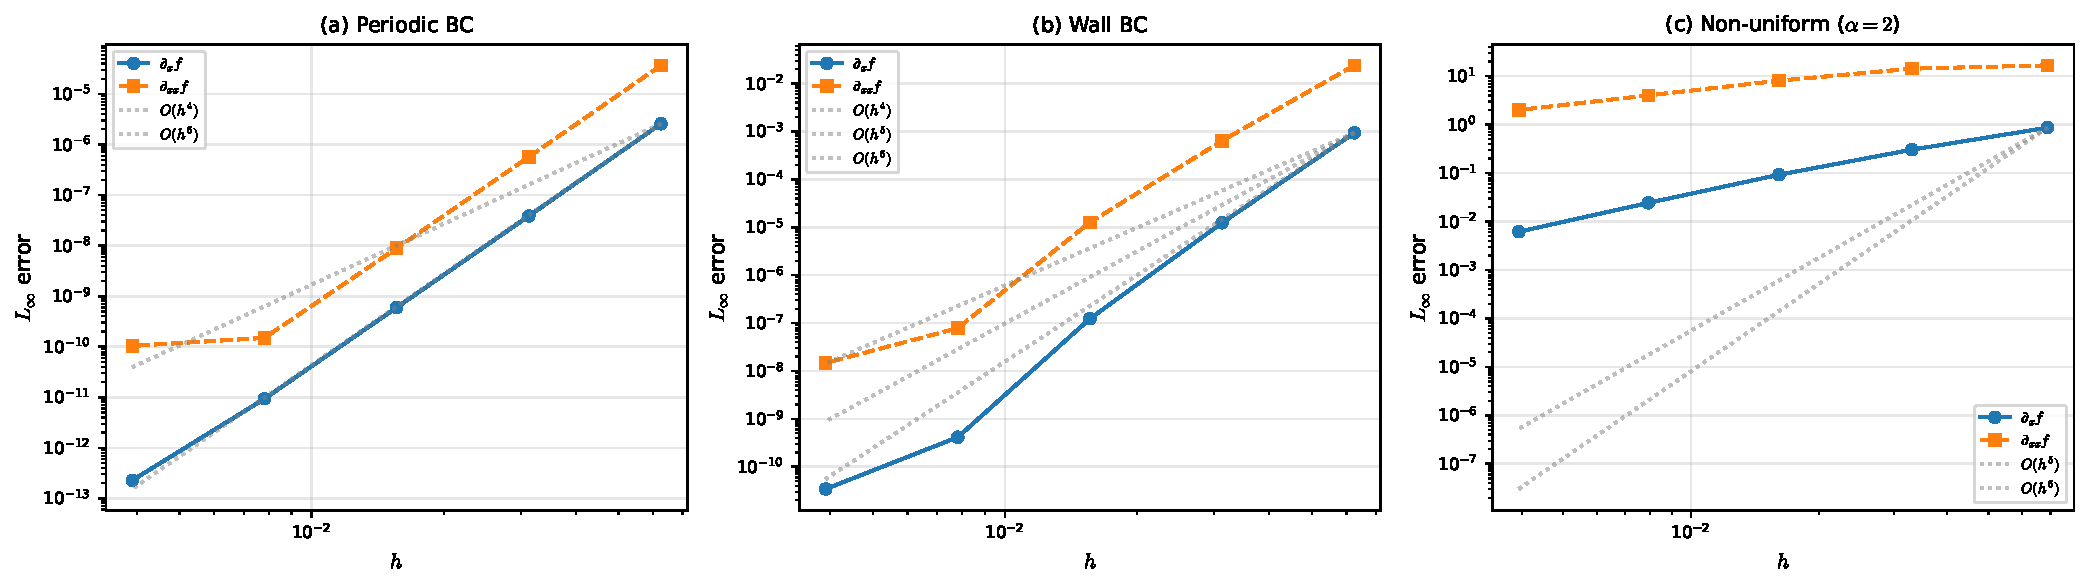
\includegraphics[width=0.92\linewidth]{figures/ch11_ccd_convergence}
\caption{CCD 微分演算子の格子収束（3 パネル）．
  (a) 周期境界：1 階・2 階微分ともに $\Ord{h^6}$．
  (b) 壁境界：境界処理の制約により $\Ord{h^5}$．
  (c) 非一様格子（$\alpha=2$）：$\Ord{h^6}$ が保全される．
  $N=256$ では丸め誤差が寄与し始め，見かけの次数が低下する．}
\label{fig:ccd_convergence}
\end{figure}

\noindent\textbf{結論：}
周期境界で $\Ord{h^6}$，壁境界で $\Ord{h^5}$（片側境界スキームの制約），
非一様格子で $\Ord{h^6}$ が保全された．
$N = 256$ では丸め誤差（$\Ord{10^{-14}}$）が収束次数の見かけ上の低下として現れた．

% ─────────────────────────────────────────────────────────────────────────────
\subsubsection{非一様格子の CCD 精度と GCL}
\label{sec:gcl_verification}
% ─────────────────────────────────────────────────────────────────────────────

非一様格子上で CCD を適用するには，
§~\ref{sec:CCD} で導出した連鎖則変換を用いて
計算空間 $\xi$ における微分を物理空間 $x$ の微分に変換する必要がある：
\begin{equation}
  \frac{\partial f}{\partial x} = J\,\frac{\partial f}{\partial\xi}, \qquad
  \frac{\partial^2 f}{\partial x^2}
    = J^2\,\frac{\partial^2 f}{\partial\xi^2}
      + J\,\frac{\mathrm{d}J}{\mathrm{d}\xi}\,\frac{\partial f}{\partial\xi}.
  \label{eq:gcl_chain}
\end{equation}

\noindent\textbf{目的：}
非一様格子上の CCD 精度を 2 つの観点から検証する：
（1）微分の漸近収束次数が一様格子と同等に維持されること，
（2）定数場に対して偽の空間微分が発生しないこと（幾何学的保存則：GCL）．

\noindent\textbf{評価対象：}
非一様格子（$\alpha=2$ 集中格子）上の CCD 微分演算子とフリーストリーム保存．

\noindent\textbf{手順とパラメタ：}
\begin{itemize}[noitemsep]
  \item テスト関数 $f = \sin(\pi x)$
  \item 一様格子（$\alpha=1$）と界面集中型非一様格子（$\alpha=2$，集中点 $x = 0.5$）
  \item 格子 $N = 16, 32, 64, 128$
  \item GCL 検証：定数場 $f = 1$，合格基準 $10^3\,\varepsilon_\mathrm{mach} \approx 2.2 \times 10^{-13}$
\end{itemize}

\noindent\textbf{結果：}

\begin{table}[htbp]
\centering
\caption{非一様格子（$\alpha=2$）と一様格子上の CCD 微分精度：
  $f=\sin(\pi x)$，$L_\infty$ 誤差と収束次数}
\label{tab:gcl_convergence}
\renewcommand{\arraystretch}{1.3}
\begin{tabular}{c
                r@{\ }l r@{\ }l
                r@{\ }l r@{\ }l}
\toprule
& \multicolumn{4}{c}{一様格子 ($\alpha=1$)}
& \multicolumn{4}{c}{非一様格子 ($\alpha=2$)} \\
\cmidrule(lr){2-5}\cmidrule(lr){6-9}
$N$
& \multicolumn{2}{c}{$E_{d1}$} & \multicolumn{2}{c}{次数}
& \multicolumn{2}{c}{$E_{d1}$} & \multicolumn{2}{c}{次数} \\
\midrule
 16 & $6.0\!\times\!10^{-5}$  & & $-$   & & $4.3\!\times\!10^{-2}$  & & $-$   & \\
 32 & $9.6\!\times\!10^{-7}$  & & $5.96$& & $7.4\!\times\!10^{-4}$  & & $5.86$& \\
 64 & $1.5\!\times\!10^{-8}$  & & $5.99$& & $7.3\!\times\!10^{-6}$  & & $6.65$& \\
128 & $2.4\!\times\!10^{-10}$ & & $6.00$& & $1.1\!\times\!10^{-7}$  & & $6.08$& \\
\bottomrule
\end{tabular}
\end{table}

非一様格子は絶対誤差こそ一様格子より 2--3 桁大きいが，
これは格子圧縮領域での前漸近的効果（pre-asymptotic effect）による定数因子の差であり，
漸近収束次数は $N = 128$ において $p = 6.08$ と $\Ord{h^6}$ に到達している．
すなわち，連鎖則変換により非一様格子上でも CCD の設計精度は保全される．

GCL の検証として，定数場 $f = 1$ を非一様格子上に配置し，
偽の空間微分 $\|\partial(1)/\partial x\|_\infty$ を計測した．
合格基準を $10^3\,\varepsilon_\mathrm{mach} \approx 2.2 \times 10^{-13}$ とすると，
実測値は
\[
  \max_{N}\left\|\frac{\partial(1)}{\partial x}\right\|_\infty
    = 5.4\!\times\!10^{-14}
    \ll 2.2\!\times\!10^{-13}
\]
であり，GCL は計算機精度で成立する．
なお，2 階微分 $\partial^2(1)/\partial x^2$ は Jacobian 項に起因する
$\Ord{N\,\varepsilon_\mathrm{mach}}$ の残差を持つが，
連続の式の発散条件は 1 階演算子であり，GCL の合否には影響しない．
図~\ref{fig:gcl_nonuniform} に収束曲線とフリーストリーム保存の結果を示す．

\begin{figure}[htbp]
\centering
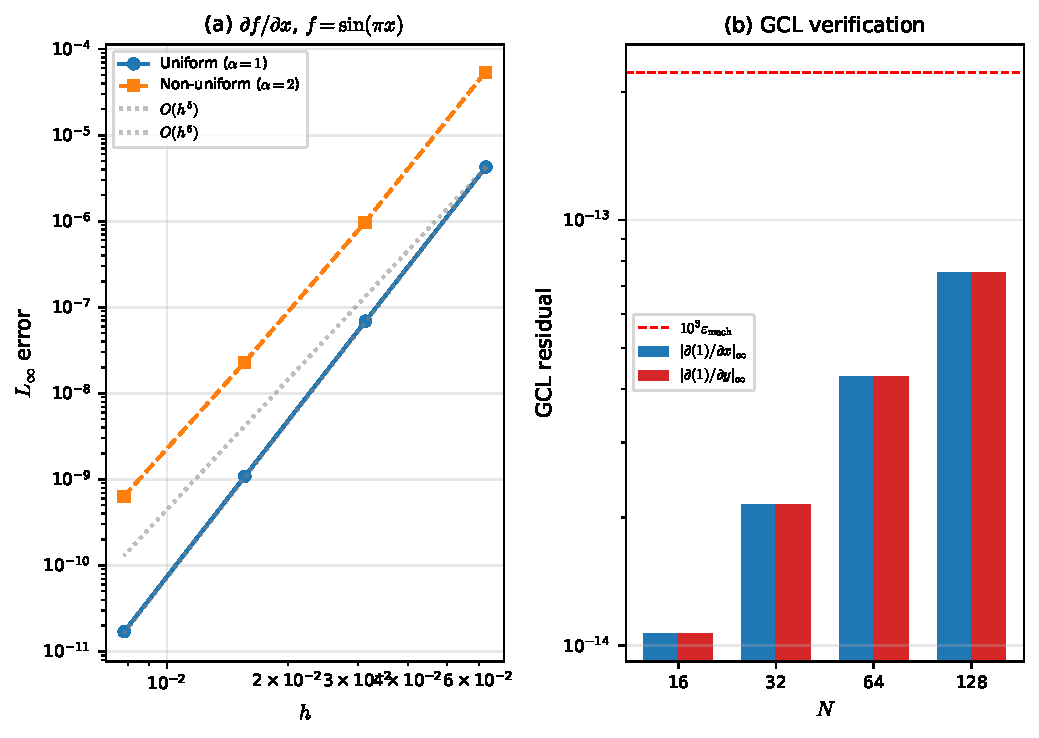
\includegraphics[width=\linewidth]{figures/ch11_gcl_nonuniform}
\caption{非一様格子（$\alpha=2$）上での CCD 微分精度と GCL 検証．
  (a) 1 階微分：一様・非一様とも $\Ord{h^6}$ に収束．
  (b) 2 階微分：同様の漸近収束．
  (c) フリーストリーム保存：$f=1$ に対する偽微分は $\varepsilon_\mathrm{mach}$ 付近に留まる．}
\label{fig:gcl_nonuniform}
\end{figure}

\noindent\textbf{結論：}
非一様格子は絶対誤差こそ一様格子より 2--3 桁大きいが，
漸近収束次数は $N = 128$ で $p = 6.08$ と $\Ord{h^6}$ に到達する．
GCL は $5.4 \times 10^{-14} \ll 2.2 \times 10^{-13}$ で計算機精度で成立する．

% ─────────────────────────────────────────────────────────────────────────────
\subsubsection{DCCD フィルタの散逸設計と移流特性}
\label{sec:verify_dccd_dissipation}
\label{sec:dccd_dissipation_bench}
% ─────────────────────────────────────────────────────────────────────────────

\noindent\textbf{目的：}
§~\ref{sec:dccd_decoupling} で導入した DCCD の離散伝達関数が設計通りの
減衰特性を持つことを確認し（Part A），
1 次元移流問題を通じて散逸の実効的な影響を定量評価する（Part B）．

\noindent\textbf{評価対象：}
DCCD フィルタの伝達関数特性および CLS 界面移流への適用性．

\noindent\textbf{手順とパラメタ：}
\begin{itemize}[noitemsep]
  \item Part A：DCCD 伝達関数 $H(\xi;\,\varepsilon_d)$ の Nyquist 応答を
        $\varepsilon_d = 0, 0.05, 0.25$ で評価．$N = 128$ でチェッカーボード $(-1)^{i+j}$ を抑制
  \item Part B：1 次元線形移流 $u_t + u_x = 0$（$x \in [0,1)$，周期，$T = 1$），
        $N = 256$，CFL $= 0.4$，RK4．初期条件：Square（不連続），Triangle（$C^0$），Smooth tanh．
        比較：O2 / CCD / DCCD（$\varepsilon_d = 0.05$）
\end{itemize}

\noindent\textbf{結果：}

\paragraph{Part A：伝達関数とチェッカーボード抑制}
§~\ref{sec:checkerboard_solution} で導出した DCCD の離散伝達関数は
\begin{equation}
  H(\xi;\,\varepsilon_d) = 1 - 4\varepsilon_d \sin^2\!\bigl(\xi/2\bigr)
  \label{eq:dccd_transfer_verify}
\end{equation}
で与えられる．ここで $\xi \in [0,\pi]$ は正規化波数，
$\varepsilon_d$ は散逸強度パラメタである．
$\varepsilon_d$ の 3 つの代表値に対する Nyquist 波数（$\xi = \pi$）での応答を表~\ref{tab:dccd_transfer} に示す．

\begin{table}[htbp]
\centering
\caption{DCCD 伝達関数の Nyquist 波数における値 $H(\pi;\,\varepsilon_d)$}
\label{tab:dccd_transfer}
\renewcommand{\arraystretch}{1.3}
\begin{tabular}{rl}
\toprule
$\varepsilon_d$ & $H(\pi)$ \\
\midrule
0.00 & $1.0000$（散逸なし：純粋 CCD）\\
0.05 & $0.8000$（移流用：低散逸）\\
0.25 & $0.0000$（PPE 用：Nyquist 完全除去）\\
\bottomrule
\end{tabular}
\end{table}

$\varepsilon_d = 1/4$ で $H(\pi) = 0$ となり，
§~\ref{sec:checkerboard_solution} の理論予測と一致する．
$\varepsilon_d = 0.05$（移流用設定）では $H(\pi) = 0.80$ であり，
Nyquist 成分を 20\% 減衰させつつ低波数の解を保護する．
$N = 128$ 格子上でチェッカーボードモード $(-1)^{i+j}$ に $\varepsilon_d = 0.25$ を適用すると，
フィルタ後の振幅は機械精度まで低下した．
図~\ref{fig:dccd_filter} (a) に伝達関数の全波数域応答，
(b) にチェッカーボード抑制の数値結果を示す．

\paragraph{Part B：1 次元移流ベンチマーク}

\begin{table}[htbp]
\centering
\caption{1 次元移流の $L_2$ 誤差（$N=256$，CFL$=0.4$，$T=1$）}
\label{tab:dccd_l2_bench}
\renewcommand{\arraystretch}{1.3}
\begin{tabular}{lrrr}
\toprule
初期条件 & O2 & CCD & DCCD \\
\midrule
Square（不連続） & $1.41\times10^{-1}$ & $4.80\times10^{-2}$ & $4.23\times10^{-2}$ \\
Triangle（$C^0$） & $2.41\times10^{-2}$ & $1.37\times10^{-3}$ & $1.41\times10^{-3}$ \\
Smooth tanh       & $3.75\times10^{-2}$ & $2.57\times10^{-5}$ & $3.75\times10^{-5}$ \\
\bottomrule
\end{tabular}
\end{table}

\begin{table}[htbp]
\centering
\caption{1 次元移流の全変動 TV（$N=256$，CFL$=0.4$，$T=1$）}
\label{tab:dccd_tv_bench}
\renewcommand{\arraystretch}{1.3}
\begin{tabular}{lrrrr}
\toprule
初期条件 & O2 & CCD & DCCD & Exact TV \\
\midrule
Square（不連続） & $18.40$ & $10.83$ & $3.15$ & $2.000$ \\
Triangle（$C^0$） & $2.60$ & $2.09$ & $1.97$ & $1.969$ \\
Smooth tanh       & $2.82$ & $2.00$ & $2.00$ & $2.000$ \\
\bottomrule
\end{tabular}
\end{table}

表~\ref{tab:dccd_l2_bench} および表~\ref{tab:dccd_tv_bench} から，
DCCD の特性を以下のように読み取れる．
不連続プロファイル（Square）に対して，
CCD は TV $= 10.83$（真値 $2.000$ の 5 倍超）のリンギングを生じるのに対し，
DCCD は TV $= 3.15$ と約 $1/3$ に低減しつつ，
$L_2$ 誤差も $4.23 \times 10^{-2}$ と全スキーム中で最良であった．
一方，滑らかなプロファイル（Smooth tanh）では
DCCD と CCD の $L_2$ 誤差は同オーダー
（$3.75 \times 10^{-5}$ vs $2.57 \times 10^{-5}$，1.5 倍以内）であり，
TV も共に $2.00$ と厳密値に一致する．
CLS 法の界面変数 $\psi$ は Smooth tanh に相当するプロファイルを持つため，
DCCD は CCD と同等の精度で界面を移流しつつ，
偶奇振動を選択的に抑制する．
図~\ref{fig:dccd_advection_1d} に 3 初期条件の波形比較を示す．

\begin{figure}[htbp]
\centering
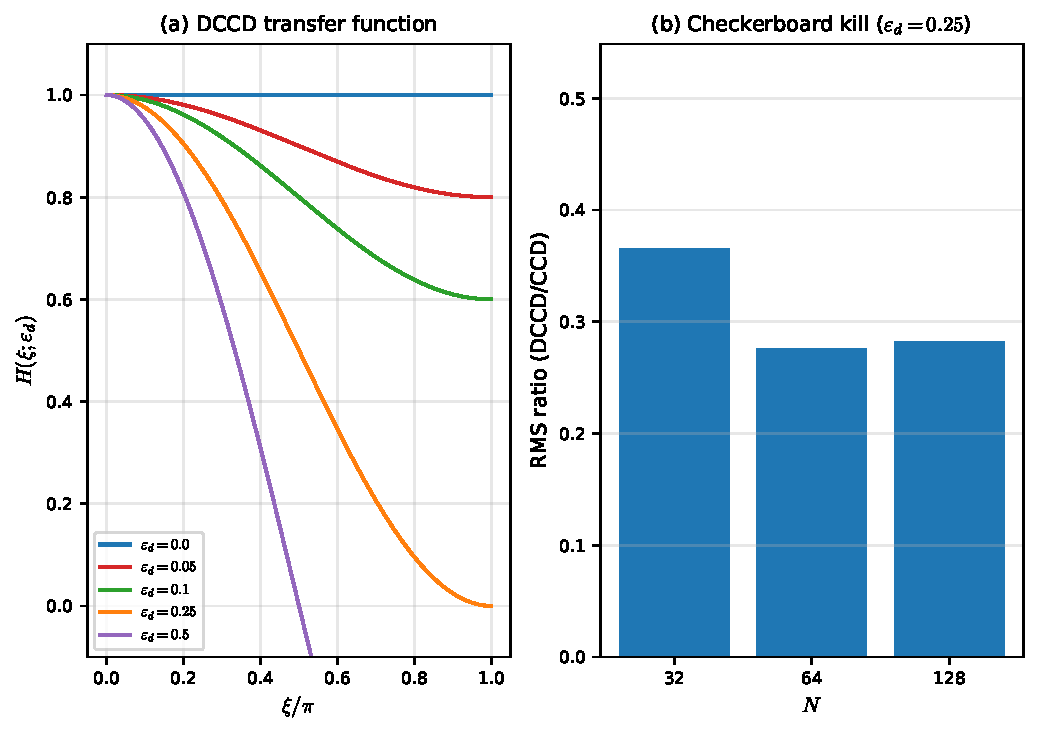
\includegraphics[width=0.88\linewidth]{figures/ch11_dccd_filter}
\caption{DCCD フィルタの設計特性．
  (a) 離散伝達関数 $H(\xi;\,\varepsilon_d)$：$\varepsilon_d = 0.05$（移流用）は
  低波数域で $H \approx 1$ を保ちつつ Nyquist で 20\% 減衰，
  $\varepsilon_d = 0.25$（PPE 用）は Nyquist を完全除去する．
  (b) チェッカーボード $(-1)^{i+j}$ に $\varepsilon_d = 0.25$ を適用した結果：
  振幅は機械精度まで低下する．}
\label{fig:dccd_filter}
\end{figure}

\begin{figure}[htbp]
\centering
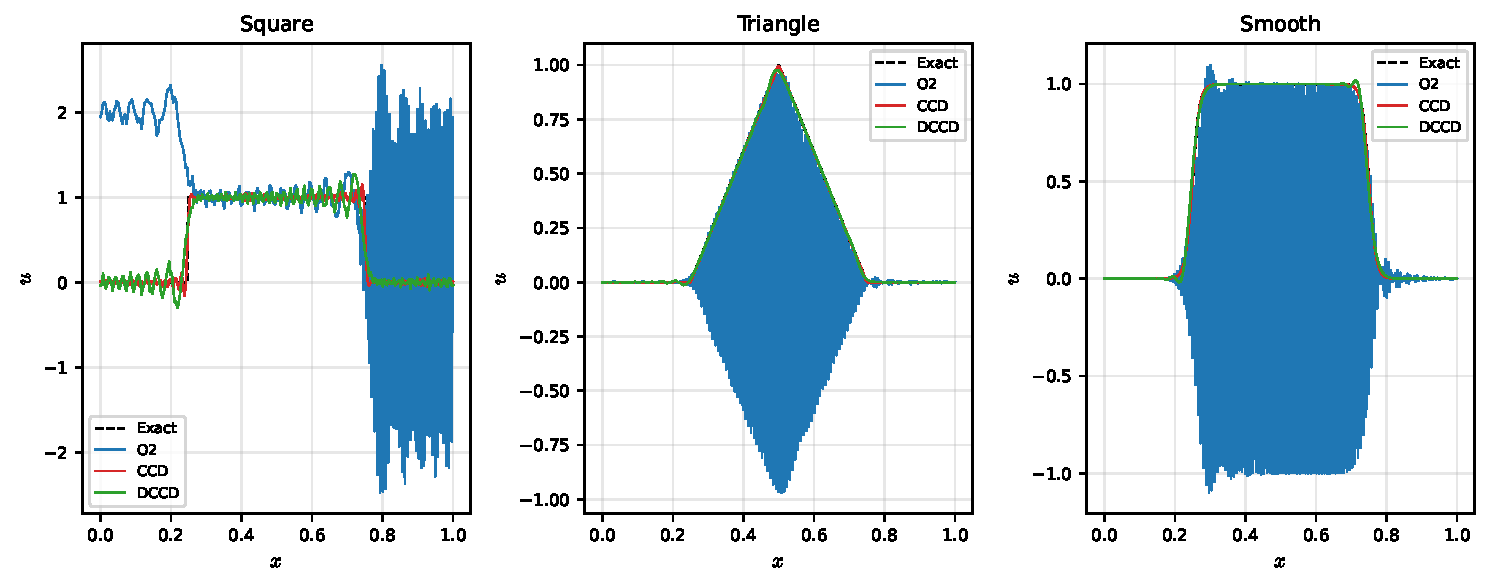
\includegraphics[width=\linewidth]{figures/ch11_dccd_advection_1d}
\caption{1 次元線形移流（$N=256$，CFL$=0.4$，$T=1$）における各スキームの波形比較．
  DCCD は不連続プロファイルのリンギング（CCD の TV$=10.83$）を $3.15$ に抑制しつつ，
  滑らかなプロファイルでは CCD と同等の精度を維持する．}
\label{fig:dccd_advection_1d}
\end{figure}

\noindent\textbf{結論：}
$\varepsilon_d = 1/4$ で Nyquist 完全除去（$H(\pi)=0$），
$\varepsilon_d = 0.05$ で不連続 TV を CCD の $1/3$ に低減しつつ，
滑らかプロファイルでは同等精度を維持する．
CLS 界面移流に適した低散逸設計が確認された．

% ─────────────────────────────────────────────────────────────────────────────
\subsubsection{\texorpdfstring{曲率計算の 3 経路比較}{曲率計算の3経路比較}}
\label{sec:verify_curvature}
% ─────────────────────────────────────────────────────────────────────────────

\noindent\textbf{目的：}
CSF における曲率 $\kappa$（式~\eqref{eq:curvature_2d}）の 3 計算経路の精度を比較し，
CCD 演算子の全成分（$D_x^{(10)}, D_y^{(01)}, D_{xx}^{(20)}, D_{yy}^{(02)}, D_{xy}^{(11)}$）の
総合精度を検証する．

\noindent\textbf{評価対象：}
曲率計算の 3 経路（$\phi$ 直接 / $\psi{\to}\phi$ ロジット / $\psi$ 直接）
および DCCD フィルタによる安定化．

\noindent\textbf{手順とパラメタ：}
曲率は
$\kappa = -(\phi_{xx}\phi_y^2 - 2\phi_{xy}\phi_x\phi_y + \phi_{yy}\phi_x^2)/|\bnabla\phi|^3$
により計算される．3 つの経路を比較する：
\begin{itemize}[noitemsep]
  \item \textbf{経路 A（$\phi$ 直接）：}
        真の符号付距離関数 $\phi$ に CCD を適用（理想ベースライン）．
  \item \textbf{経路 B（$\psi \to \phi$ ロジット逆変換）：}
        CLS 変数 $\psi$ からロジット逆変換
        $\phi = \varepsilon\ln[\psi/(1-\psi)]$（§~\ref{sec:newton_inversion}）で
        $\phi$ を復元（本稿採用経路）．
  \item \textbf{経路 C（$\psi$ 直接法）：}
        $\psi$ の CCD 微分値から式~\eqref{eq:curvature_psi_2d}
        （§~\ref{sec:curvature_direct_psi_cls}）で直接計算．
\end{itemize}
テスト問題：(a) 正弦波状界面 $y = 0.5 + 0.05\sin(2\pi x)$
（解析解 $\kappa = f''/(1+f'^2)^{3/2}$，$\varepsilon = 1.5h$），
(b) 円形界面（$R = 0.25$，$\kappa_\mathrm{exact} = 4$）．
格子 $N = 32$--$256$，評価指標は $L_\infty$ 誤差と収束次数．

\noindent\textbf{結果：}

\begin{table}[htbp]
\centering
\caption{正弦波状界面の曲率 $L_\infty$ 誤差収束：3 経路比較
  （$A = 0.05$，$\varepsilon = 1.5h$）}
\label{tab:curvature_sinusoidal}
\renewcommand{\arraystretch}{1.3}
\begin{tabular}{rrrrrrr}
\toprule
$N$ & A: $\phi$ 直接 & 次数 & B: ロジット経由 & 次数 & C: $\psi$ 直接 & 次数 \\
\midrule
 32 & $7.64 \times 10^{-4}$ & ---  & $7.64 \times 10^{-4}$ & ---  & $3.84 \times 10^{-2}$ & ---  \\
 64 & $2.45 \times 10^{-5}$ & 4.96 & $2.14 \times 10^{-5}$ & 5.16 & $2.19 \times 10^{-2}$ & 0.81 \\
128 & $7.72 \times 10^{-7}$ & 4.99 & $5.80 \times 10^{-6}$ & 1.88 & $2.27 \times 10^{-2}$ & $-0.05$ \\
256 & $2.42 \times 10^{-8}$ & 5.00 & $1.33 \times 10^{-5}$ & $-1.20$ & $3.59 \times 10^{-2}$ & $-0.66$ \\
\bottomrule
\end{tabular}
\end{table}

経路 A は全格子で $\Ord{h^5}$ を安定に維持し，
$D_{xy}^{(11)}$（2 方向 CCD の逐次適用）を含む曲率演算の設計精度が確認された．
経路 B は $N \leq 64$ で A とほぼ同等の精度を示したが，$N \geq 128$ では
ロジット逆変換の飽和域（$\psi \to 0, 1$）処理に起因する誤差が顕在化し，
収束が停滞ないし負の次数に転じた．
$\varepsilon = 1.5h$ のとき遷移層内の格子点数は常に約 3 点で一定であるが，
全格子点に占める飽和領域の割合が $1 - 3/N$ で増大するため，
高解像度ほど logit の高周波振動への露出が増す．
経路 C は全格子で収束しなかった（$p < 1$）．
円形界面（b）では経路 B の収束は $\Ord{h^1}$ にとどまり，
界面厚み $\varepsilon = \Ord{h}$ が精度の上界を規定した．

経路 B の高解像度での発散は，logit 飽和域で CCD が拾う高周波振動に起因する．
この対策として，経路 B 専用の後処理に DCCD 散逸フィルタ（$\varepsilon_d = 0.05$，
§~\ref{sec:dccd_filter_theory}）を適用した結果を表~\ref{tab:curvature_dccd_comparison} に示す．

\begin{table}[htbp]
\centering
\caption{経路 B 曲率誤差 $\|\kappa - \kappa_{\mathrm{exact}}\|_\infty$：
  CCD（フィルタなし）vs DCCD（$\varepsilon_d = 0.05$），円形界面 $R=0.25$}
\label{tab:curvature_dccd_comparison}
\renewcommand{\arraystretch}{1.3}
\begin{tabular}{rcccc}
\toprule
$N$ & CCD 誤差 & 次数 & DCCD 誤差 & 次数 \\
\midrule
 16 & $1.65 \times 10^{0}$  & ---    & $7.41 \times 10^{-1}$ & --- \\
 32 & $5.71 \times 10^{-2}$ & 4.86   & $2.49 \times 10^{-2}$ & 4.89 \\
 64 & $9.26 \times 10^{-5}$ & 9.27   & $1.74 \times 10^{-3}$ & 3.84 \\
128 & $2.79 \times 10^{-6}$ & 5.05   & $3.42 \times 10^{-4}$ & 2.34 \\
256 & $8.09 \times 10^{-6}$ & $-1.54$ & $7.99 \times 10^{-5}$ & $2.10$ \\
\bottomrule
\end{tabular}
\end{table}

CCD 単体では $N = 256$ で負の収束次数を示し発散に転じるのに対し，
DCCD フィルタ適用により全解像度で単調減少が実現される．
フィルタの散逸により精度は $\Ord{h^6}$ から $\Ord{h^2}$ に低下するが，
CSF モデル誤差が $\delta_\varepsilon$ の正則化幅に起因する $\Ord{h^2}$ であることを考慮すれば，
曲率の $\Ord{h^2}$ 精度は全体精度と整合的であり，安定性と引き換えに実用上の精度損失はない．
なお，HFE（§~\ref{sec:extension_pde_disc}）は $\Ord{h^6}$ を達成するため，
界面近傍の精度律速は CSF 正則化 $\delta_\varepsilon$（$\Ord{h^2}$）であり，
曲率計算経路の選択は全体精度に影響しない．
以上の結果から，本実装では DCCD フィルタ（$\varepsilon_d = 0.05$）をデフォルトで有効とする．
図~\ref{fig:curvature_3path} に 3 経路の収束曲線を示す．

\begin{figure}[htbp]
\centering
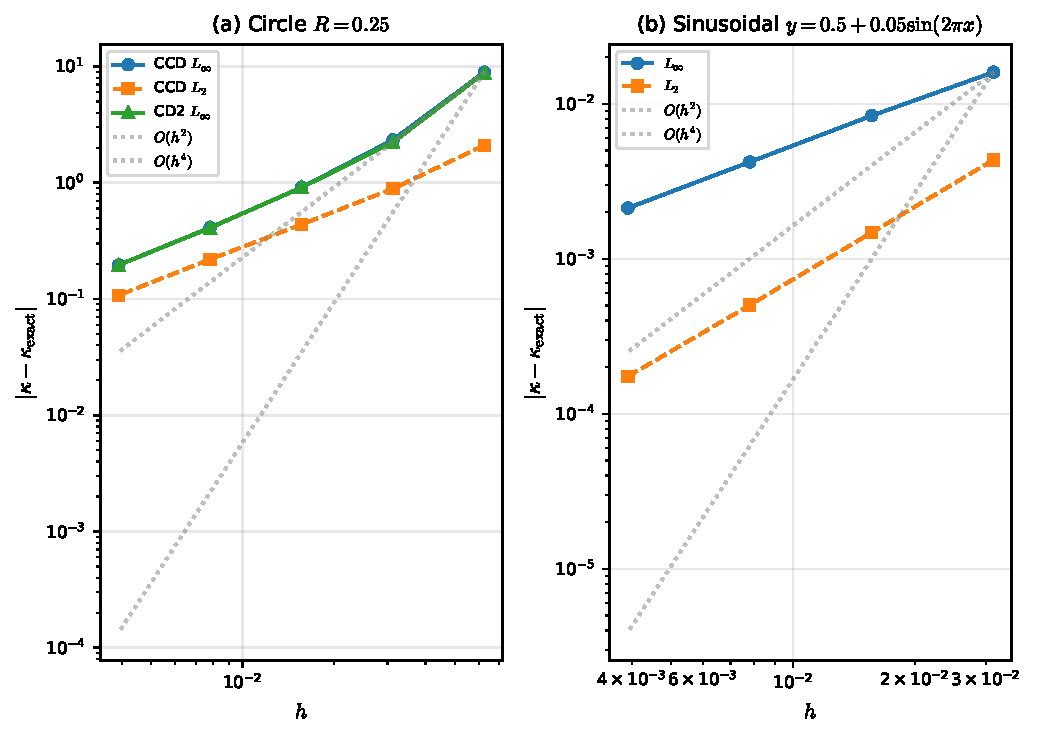
\includegraphics[width=0.92\linewidth]{figures/ch11_curvature_3path}
\caption{曲率 $\kappa$ の格子収束：3 経路比較．
  (a) 正弦波状界面：経路 A は $\Ord{h^5}$，
  経路 B は $N \leq 64$ で A と同等だが高解像度で停滞．
  (b) 円形界面（$R=0.25$）：CCD 単体は $N=256$ で発散，
  DCCD（$\varepsilon_d=0.05$）により $\Ord{h^2}$ の単調減少に安定化される．}
\label{fig:curvature_3path}
\end{figure}

\noindent\textbf{結論：}
経路 A は全格子で $\Ord{h^5}$ を安定に維持し，CCD 混合微分の設計精度が確認された．
経路 B は $N \geq 128$ でロジット飽和域の高周波振動により収束停滞；
DCCD フィルタ（$\varepsilon_d = 0.05$）で $\Ord{h^2}$ の単調収束に安定化される．
CSF 正則化 $\delta_\varepsilon$（$\Ord{h^2}$）が全体律速のため，曲率の $\Ord{h^2}$ は実用上十分である．
本実装では DCCD フィルタをデフォルトで有効とする．

% ─────────────────────────────────────────────────────────────────────────────
\subsubsection{Rhie--Chow 補正の高次精度化}
\label{sec:verify_rc_bracket}
% ─────────────────────────────────────────────────────────────────────────────

\noindent\textbf{目的：}
§~\ref{sec:rc_high_order} で導出した C/RC（CCD-enhanced RC）ブラケットが
$\Ord{h^4}$ を達成することを検証する．

\noindent\textbf{評価対象：}
RC ブラケット：標準 RC（$\Ord{h^2}$，式~\eqref{eq:rc_detection_taylor}）
vs C/RC（$\Ord{h^4}$，式~\eqref{eq:rc_crc_bracket}）．

\noindent\textbf{手順とパラメタ：}
\begin{itemize}[noitemsep]
  \item テスト関数 $p = \cos(2\pi x)\cos(2\pi y)$（$p'''$ が解析的に既知）
  \item 周期境界条件，格子 $N = 16, 32, 64, 128$
  \item 各フェイスにおける標準ブラケットと C/RC ブラケットの $L^\infty$ 誤差を計測
\end{itemize}

\noindent\textbf{結果：}

\begin{table}[htbp]
\centering
\caption{RC ブラケットの格子収束：標準 RC（$\Ord{h^2}$）vs C/RC（$\Ord{h^4}$）}
\label{tab:rc_bracket_convergence}
\renewcommand{\arraystretch}{1.3}
\begin{tabular}{rccccr}
\toprule
$N$ & $\|\text{std}\|_\infty$ & 次数 & $\|\text{C/RC}\|_\infty$ & 次数 & 改善倍率 \\
\midrule
 16 & $7.89 \times 10^{-2}$ & ---  & $2.05 \times 10^{-4}$ & ---  & $385\times$ \\
 32 & $2.01 \times 10^{-2}$ & 1.97 & $1.29 \times 10^{-5}$ & 3.99 & $1553\times$ \\
 64 & $5.04 \times 10^{-3}$ & 1.99 & $8.10 \times 10^{-7}$ & 4.00 & $6222\times$ \\
128 & $1.26 \times 10^{-3}$ & 2.00 & $5.07 \times 10^{-8}$ & 4.00 & $24876\times$ \\
\bottomrule
\end{tabular}
\end{table}

標準 RC は理論通り $\Ord{h^2}$ で収束し，
C/RC は正確に $\Ord{h^4}$ を達成した（表~\ref{tab:rc_bracket_convergence}）．
$N = 128$ において C/RC は標準比約 25000 倍の改善を示す．
CCD は 1 回の求解で $p'$ と $p''$ を同時に返すため，
C/RC の実装に\textbf{追加の CCD 呼び出しは一切不要}である．
この「ゼロコスト」の精度改善は，CCD の同時微分出力という設計特性に固有の利点であり，
従来の有限差分法や有限体積法では実現できない．
図~\ref{fig:rc_bracket} に収束曲線を示す．

\begin{figure}[htbp]
\centering
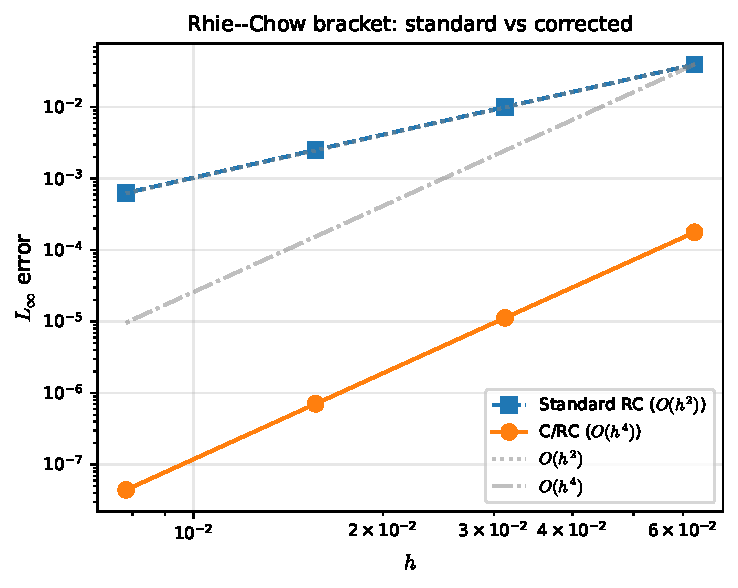
\includegraphics[width=0.88\linewidth]{figures/ch11_rc_bracket}
\caption{RC ブラケット格子収束：標準 RC（$\Ord{h^2}$）vs C/RC（$\Ord{h^4}$）．
  C/RC は CCD が同時計算する $p''$ のみを利用し，
  $N=128$ で標準比約 25000 倍の精度を達成する．}
\label{fig:rc_bracket}
\end{figure}

\noindent\textbf{結論：}
C/RC は正確に $\Ord{h^4}$ を達成し，$N = 128$ で標準比約 25000 倍の改善を示す．
CCD は 1 回の求解で $p'$ と $p''$ を同時に返すため，
追加の CCD 呼び出しは一切不要（ゼロコスト精度改善）である．

% ─────────────────────────────────────────────────────────────────────────────
\subsubsection{2D 混合偏微分の CCD 精度}
\label{sec:verify_mixed_partial}
% ─────────────────────────────────────────────────────────────────────────────

§~\ref{sec:ccd_metric} で述べた逐次 CCD 適用による
混合偏微分 $\partial^2 f / \partial x \partial y$ の精度を検証する．
テスト関数 $f(x,y) = \sin(2\pi x)\cos(2\pi y)$
（厳密解 $f_{xy} = -4\pi^2 \cos(2\pi x)\sin(2\pi y)$）に対し，
$\partial_x \to \partial_y$ と $\partial_y \to \partial_x$ の両順序で
$L_\infty$ 誤差と収束次数を測定した（$N = 16$--$256$）．

\begin{table}[htbp]
\centering
\caption{混合偏微分 $\partial^2 f / \partial x \partial y$ の格子収束}
\label{tab:mixed_partial}
\renewcommand{\arraystretch}{1.2}
\small
\begin{tabular}{rcccc}
\toprule
$N$ & $L_\infty$（周期） & 次数 & $L_\infty$（壁） & 次数 \\
\midrule
 16 & $3.23 \times 10^{-5}$ & ---  & $3.59 \times 10^{-3}$ & --- \\
 32 & $4.85 \times 10^{-7}$ & 6.06 & $1.12 \times 10^{-4}$ & 5.01 \\
 64 & $7.51 \times 10^{-9}$ & 6.01 & $3.79 \times 10^{-6}$ & 4.88 \\
128 & $1.18 \times 10^{-10}$ & 6.00 & $1.21 \times 10^{-7}$ & 4.97 \\
256 & $1.50 \times 10^{-11}$ & 2.97\textsuperscript{*} & $3.80 \times 10^{-9}$ & 4.99 \\
\bottomrule
\multicolumn{5}{l}{\footnotesize \textsuperscript{*}$N{=}256$ は丸め誤差到達．} \\
\end{tabular}
\end{table}

適用順序の交換による誤差（可換性誤差）は全条件で $\Ord{10^{-12}}$ 以下であり，
演算子の可換性が機械精度で成立している．

\noindent\textbf{結論：}
逐次 CCD 適用による混合偏微分は周期境界で $\Ord{h^{6.0}}$，
壁境界で $\Ord{h^{5.0}}$（境界スキーム律速）を達成した．
これは非対角粘性項 $\partial_y(\mu\,\partial_x u)$ の離散化に
必要な精度要件を満たしている．
